% This is samplepaper.tex, a sample chapter demonstrating the
% LLNCS macro package for Springer Computer Science proceedings;
% Version 2.20 of 2017/10/04
%
\documentclass[runningheads]{llncs}
%
\usepackage{float}
\usepackage{graphicx}
\usepackage{tablefootnote}
\usepackage{longtable}
% Used for displaying a sample figure. If possible, figure files should
% be included in EPS format.
%
% If you use the hyperref package, please uncomment the following line
% to display URLs in blue roman font according to Springer's eBook style:
% \renewcommand\UrlFont{\color{blue}\rmfamily}
\let\labelitemi\labelitemii

\setlength{\arrayrulewidth}{0.5mm}
\setlength{\tabcolsep}{18pt}
\renewcommand{\arraystretch}{1.5}


\begin{document}
%
\title{DropShop }%\thanks{Supported by organization x.}
\subtitle{Whitepaper v.1.0}
%
%\titlerunning{Abbreviated paper title}
% If the paper title is too long for the running head, you can set
% an abbreviated paper title here
%
\author{Ryan D. Miller, Colin Steidtmann \and Seung Y. Lee}
%
\authorrunning{R.D. Miller et al.}
% First names are abbreviated in the running head.
% If there are more than two authors, 'et al.' is used.
%
\institute{Hackathon Team\\
\email{\{Ryan.D.Miller05,colinsteidtmann,seung.youn.lee\}@gmail.com}}
%
\maketitle              % typeset the header of the contribution
%

\begin{abstract}
Verified randomness allows for blockchains to fairly select winning participants in probability-driven events between decentralized parties.  Blockchain-based lossless lotteries are an example of this capability and offer numerous advantages over traditional lotteries around transparency and accessibility.  Most notably, they eliminate risk, as a winner’s rewards are generated through DeFi protocols and Yield Farming, rather than as a claim on the other participants' stakes; non-winners get their stake back.

DropShop proposes to use this same principle towards limited edition product drops.  These drops have existed for many years in the form of event tickets, but most recently they have been popularized by apparel and even technology companies for physical goods, such as Sneakers, Bags, and gaming systems.  Currently, these drops are dominated by rent-seeking middlemen using bots and other methods to capture as much of the product as they can for resale.  As such, we seek to democratize these drops using a decentralized lottery where product supporters can increase their odds through brand interaction, promotion and community building.


\keywords{ Lottery \and Rare Items \and DeFi \and Smart contracts \and Blockchain \and Ethereum \and ChainLink.}
\end{abstract}
%
%
%
\section{Introduction - Limited Release Product Drops}\label{intro-sec}

\subsection{Summary}
Limited release product drops are a key marketing strategy for any product that can generate brand equity from ‘hype’ – a type of grassroots marketing value.  However, these drops are vulnerable to manipulation, particularly by automated Bots who buy up a large portion of the limited product.  This inflates the product’s price on the secondary market, with Bots capturing most of this value.  

The potential for brand harm by Bots pricing out some consumers is often outweighed by the additional value to the brand, as resale markets act to accelerate hype.

A better solution to the current paradigm would shift the capture of resale value from purely rent seeking middlemen (the Bots) to those who value the brand or service most – the brand’s biggest supporters.


\subsection{History}
Yeezy sneakers, Supreme gear, PlayStation 5s, Hot NFT collections.  What do they all have in common?  They’re highly desired products with limited supply.

Once the province of event tickets such as concerts and sporting events, limited product releases – referred to as ‘Drops’ - have become a mainstay of brand marketing.  They rely on ‘Hype’ - grassroot driven excitement.  Once relegated to word of mouth in niche circles, social media technologies have brought these hushed forums into virtually every pocket with a phone and Twitter account.\cite{1}

Drops originated in Japanese streetwear brands in the 1990s before spreading to the United States, where the technique was popularized by brands like Supreme and The Hundreds.  Drops provide a way for companies to generate a steady drumbeat of press coverage and brand awareness.  In the process of shopping a drop, customers often learn everything about the brand story, or the artists that made it.  It’s powerful from the brand perspective, so much so that even large, established companies use them in between proper, fully fledged product releases.  For example, drops now play a prominent role in Nike’s direct-to-consumer strategy.\cite{2}

While sneaker companies have been one of the most visible beneficiaries of drop culture, perhaps the largest beneficiary have been resellers.  Around 50\% of all Nike sneakers that were released in the first quarter of 2021 were available on StockX (a leading reseller marketplace) and had a price premium of 50\% or more.  Cowan estimates the sneaker resale market at \$2B in the US alone, part of a larger \$24B resale market.\cite{3} 

But herein lies a downside of this marketing strategy – if a reseller gains an advantage over other customers in purchasing a limited release item, they can snatch up much of the entire drop for themselves, and thereby extract unearned value from the resale market they effectively control.


\subsection{The Problem: Rent-Seeking Using Bots} 
For years performers priced tickets below the market-clearing price, either out of fairness or out of concern for the long-term value of their brand.\cite{4}   In addition, as many tickets are given away or sold to primary channels at contracted rates, keeping premiums in check. Traditional resale markets for tickets reflected a ‘truer’ premium, but historically these were limited to smaller individual resellers whose labor added a degree of fluidity to the market – thereby adding some value to the exchange as a whole.  Think of the lone ticket scalper outside of Yankee stadium.

Beginning with the streetwear drop culture spearheaded by Supreme, this began to change.  Drop products are priced to their target consumers, but while relatively low retail prices give consumers of varying financial means an opportunity to buy, high demand for the product feeds into the resale market, and product hits the secondary market at inflated prices. For example, Supreme box logo crewnecks that originally sold for \$158 resell for a minimum of \$500.\cite{5}

These Supreme drops would occur at their physical store every Thursday, with people queuing in line sometimes for days for the chance to score a drop item.  In order to ensure drops were getting into the hands of their actual customers, limits to purchasing were enforced, and Supreme security personnel both inside and outside monitor activity to see if people trade places in line for cash, or if items were deemed being purchased purely for resale.\cite{6}

Still, this didn’t prevent resellers with the means to do so from paying individuals to wait in line for them, knowing they would more than recoup the cost in the secondary market.

However, as more retailers began offering drops online, the process that used to involve camping out has now entered the world of high-tech arbitrage - in particular, automated Bots: web scrapers, automated shopping cart ‘sniper’ bots, and login and checkout abusers.\cite{7} These Bots are run by everyone from individual 15-year-old kids sitting in a basement somewhere making \$200,000 a year reselling sneakers, to organized reseller syndicates called “cooks” who deploy professional scraping software\footnote{Cybersole, GaneshBot, and Kodai to name a few.}  to scour the website for the stock-keeping units, or SKUs, associated with new inventory. As new SKUs come online, the bots add each item associated with that unique ID number to a shopping cart, and once the sale starts, they try to complete the checkout process using a preloaded credit card or gift card information. Non-bot-using customers hate them because it’s almost impossible to check out faster than a bot can. Frequently, one or two bots buy up a large chunk of the product simply to resell it – a poor customer experience for everyone.\cite{8}

These bots have led to hugely inflated prices in a secondary market effectively controlled by rent-seeking individuals, making many of the products inaccessible to the primary customers who value them most. Nike sees this as a problem: \emph{“We are constantly looking at the best way to combat bots across our digital ecosystem. Nike is fully committed to making sure that our real, loyal consumers are the ones who get fair access to our products and that we continue to evolve best-in-class solutions in the marketplace.”}\cite{9} 

\begin{figure}[H]
\centering
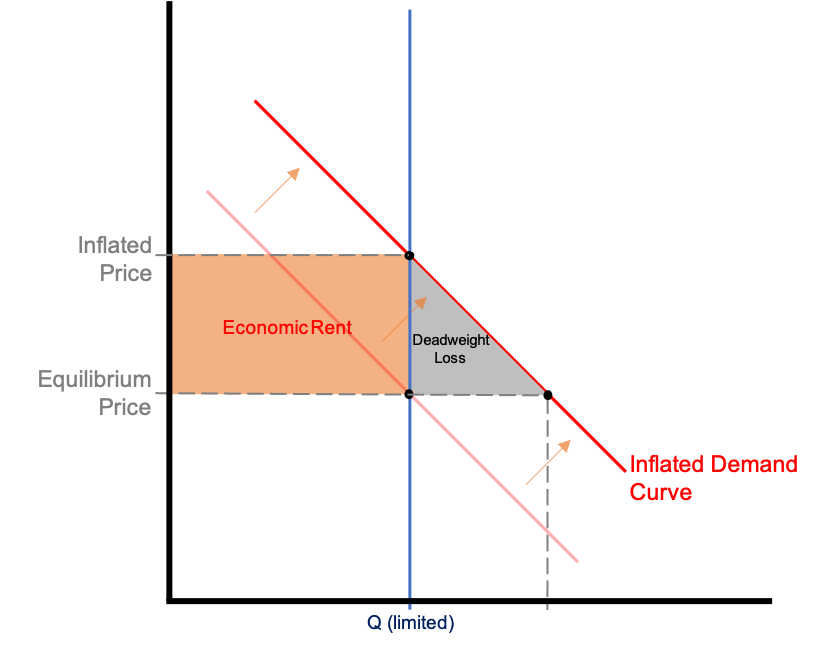
\includegraphics[scale=0.8]{Figures_and_Tables/Rent-Capture Supply&Demand.png}
\caption{Rent capture and Deadweight Loss driven by Bot-inflated Demand: Bots drive overall demand up.  With a fixed supply this creates artificial value the users of bots capture in a secondary market composed mostly of primary customers.  That artificial value is economic rent.}
\end{figure}

In 2016, Congress enacted the BOTS Act (Better Online Ticket Sales Act) attempting to legally close this loophole for event tickets.\cite{10}   But in 5 years only a single case has been brought to court by the FTC, who are tasked with enforcing the act.\cite{11}   Meanwhile, Bots are still wreaking havoc on ticket markets.  Take for instance Burning Man, whose core values are “Radical Inclusion, Diversity, and Equity”.  They admit that their 2019 public ticket sale (the last year the event was held due to COVID) was dominated by Bots.\cite{12}   That’s a direct affront to their values.

Regardless of the BOTS lack of bite, the legislation does not cover other products.  As such, companies are taking it upon themselves to combat Bots in the name of equity for their loyal consumers.  \emph{“People are still asking for transparency, and they are still frustrated and angry”.}\cite{13}

Primary retailers tried using online raffles rather than first-come first-served sales, but those too have been defeated by bots buying up all the raffle tickets.  This has led them to fighting fire with fire, utilizing anti-bot software such as Akamai, at great cost.  Akamai brings in just under \$200M a year and is growing 40\% annually.\cite{14}

It’s turned into a cat and mouse game, with Bots becoming more sophisticated in response.  Disturbingly, with the COVID-driven increase in ecommerce, and current worldwide supply chain issues, the problem with Bots is only getting worse. \emph{“People will try to jump the line and leverage automation to grab anything that has a limited inventory.  It used to be concert tickets, then purses and tennis shoes, and now it’s vaccine reservations and even more mundane things.”}\cite{14}

\subsection{Solution Attributes} 
While Bots damage customer experience, they have created a conundrum.  The inflated resale market is now integral to how drops work, as it serves as a metric for a brand’s success: higher resale price tags mean greater hype, and greater hype means a higher brand value.\cite{16}
	
Brands would prefer to replace the brand value \emph{generated by Bots inflating the market} with brand value \emph{generated as close to the customer as possible.}  Therefore, a better solution to the problem must include two key characteristics:
\begin{enumerate}
\item Eliminate the Bots, but not the resale market
\item Offer a mechanism to signal value and grow hype (must compensate for lost hype due to lower secondary market inflation).
\end{enumerate}

We propose a blockchain based platform with these solution attributes to democratize market participation, keeping primary customers in the primary market.  We call this platform \textbf{DropShop}.

\section{Paper Roadmap}\label{PaperRoadmap}

This whitepaper describes DropShop, a blockchain powered lottery platform as a solution to the problems with limited release product drops.\footnote{We speak in the art of what is possible, so certain considerations around gas and LINK optimization or the mechanics behind a multiple blockchain platform are not explored in-depth.  However future iterations of this Whitepaper, and the platform built off of its ideas, will take these considerations into detail.}   

We first give an overview of this blockchain lottery platform [Section \ref{section-LotteryOverview}] and then define the two user roles within the platform, along with their characteristics and general flows. [Section \ref{section-Users}]

Next, the paper describes the initialization and operation of the lottery itself -  parametrization, launch, and selection of winners.  It then proposes several models to incentivize all users to fulfill their obligations to the platform and each other.   [Section \ref{section-LotteryProcess}]

A basic discussion of the economics of the platform follows, highlighting its value creation and flows. [Section \ref{section-PlatformEconomics}]  

Lastly, we briefly discuss additional features, including an integrated secondary marketplace, generalizing the platform beyond Drops to other forms of user-to-user asset transactions, and evolving into a DAO.   [Section \ref{section-FutureFeaturesGrowth}]


\section{Blockchain Lottery Overview}\label{section-LotteryOverview}

When the demand for a certain good exceeds its supply, market forces raise the price of the good such that it equals the willingness to pay of those who want it most.  When the quantity of a good is highly limited, but price is variable, auctions are often the most effective mechanism for revealing an individual’s willingness to pay.\cite{17}

But in the case where both quantity \emph{and} price are fixed, such as in a limited release ‘drop’, auction mechanisms are no longer effective, as there is no differentiation among buyers whose willingness to pay is higher than the fixed price which must be set.

Most of these sales are therefore first come first serve, a model easily gamed through technology or collusion by those who seek to capture economic rent from these limited goods by buying then reselling them at inflated prices.

One method to overcome rent-seeking resellers is through a time-bounded raffle mechanism.\cite{18}   Buyers willing to pay the fixed price enter the raffle and are chosen at a set time by random chance.  However, it does not address degree of preference of each buyer, and can still be gamed by technology and collusion.

Therefore, we propose a hybrid model combining a raffle with an individual’s \textbf{Overall Preference} for a limited good.  Overall preference is one’s willingness to pay - signaled by the premium they would pay on top of the price of that good, combined with a measure of non-monetary value one is willing to exchange for the good – in this case signaled by hype-generating brand interactions.

To accomplish this, we propose a blockchain based system following the following first principles:
\begin{enumerate}
\item Anyone can create a lottery or participate in one (permissionless).
\item No centralized authority runs the platform.
\item Lottery creators have full control over the parameters of their lottery, which are fully transparent to the lottery participants.
\item Lottery outcomes are assured by verifiable randomness. 
\end{enumerate}

The first three can be made inherent to a blockchain protocol; for the last, oracles can be used for randomness and off-chain computation.  Properly designed, this system disincentivizes Bots yet incentivizes the participation of primary consumers.  These primary consumers stake money through a no-loss mechanism – either they win and automatically purchase the item at their stake price, or do not win and receive their money back.  The winners are randomly selected with their individual odds determined by the strength of their overall preferences.


\section{Users}\label{section-Users}

The \textbf{DropShop} platform is composed of two types of Users: \emph{Sponsors}, who create lotteries, and \emph{Participants}, who stake funds to win them.  As a decentralized platform, any entity in the world can be a Sponsor, and any entity in the world can be a Participant; thus, any user can be both a Sponsor and a Participant.  The interface when using the platform as a Sponsor or Participant differ greatly, although every user has access to both.  However, most users will utilize the platform as just one of these user types.

\begin{figure}[H]
\centering
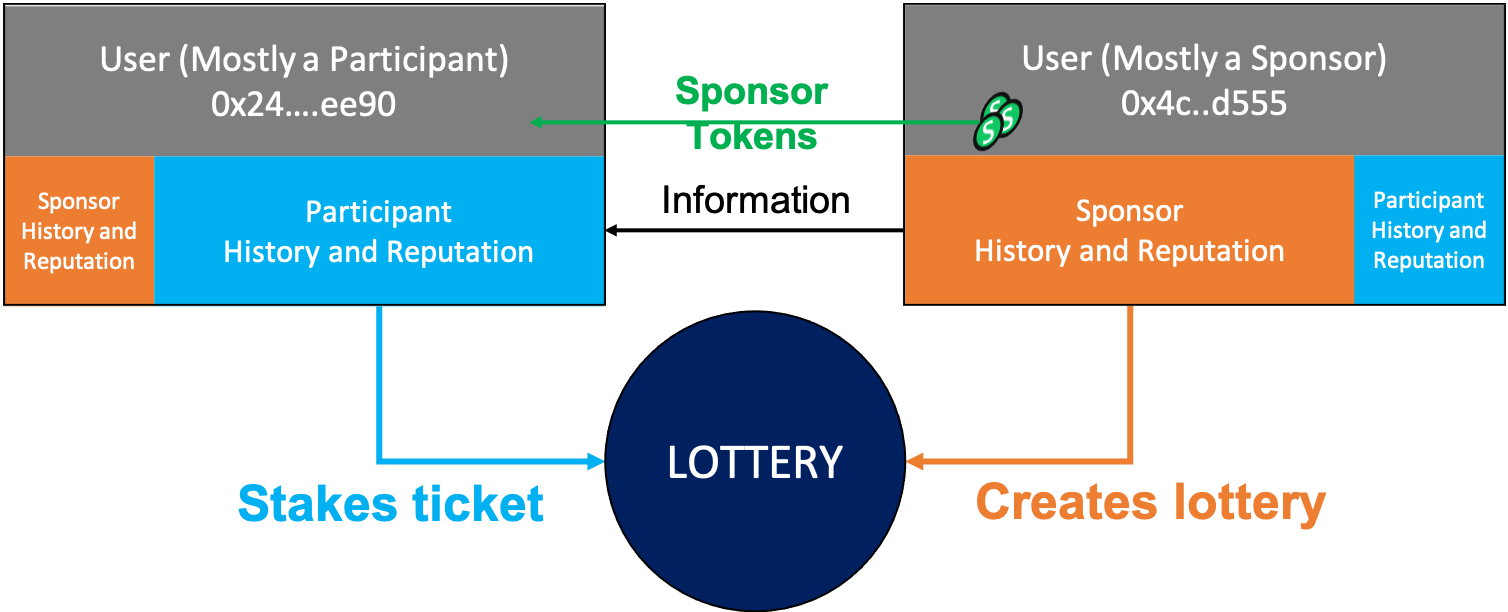
\includegraphics[scale=0.5]{Figures_and_Tables/User_Structure.png}
\caption{User Structure.}
\end{figure}

All users are permanently tied to one or more wallet addresses which serve as their primary identification within the system.  This is the only requirement for interacting with the system. However, they can add additional information tied to that wallet including a username, Avatar, and social media accounts.  This is more critical for Sponsors in order to identify themselves and their Lotteries to Participants.

\subsection{Sponsors}\label{subsection-Sponsors}
Sponsors create a lottery by defining its parameters and writing them to a smart contract.  Sponsors have full control over the parameters of their lotteries (discussed in the Lottery Process subsection \ref{subsection-CreatingLottery} below), and these parameters are completely transparent to Participants.   

Examples of Sponsors include:
\begin{itemize}
\item Clothing and Accessory Brands (Nike, Supreme, Yeezy)
\item Electronics and Gaming Platforms (Playstation, ASIC Cards)
\item Ticketed Events (Musicians, Sports Teams)
\item Certain fungible and non-fungible token releases
\item Physical Art Collections
\end{itemize}

\subsubsection{Sponsor Interface and Dashboard.}  After connecting their wallet to the system, the user accesses the Sponsor interface within the platform.  

The Sponsor Interface and Dashboard includes:
\begin{itemize}
\item User Settings 
\item Sponsor Reputational Scores
\item Lotteries in Progress, to include Collateral Locked
\item Lottery History and Metrics
\item Access to Sponsor Token smart contract (mint and distribute)
\item Access to Lottery smart contract for lottery creation
\end{itemize}

Sponsors can run as many concurrent lotteries as they like, determining the parameters for each independently.

\subsubsection{Sponsor Tokens}  Sponsors can mint ‘Sponsor Tokens’ and issue them to Participants.  Sponsors can create and issue as many types of tokens at they like (such as a general token, a Spring collection token, etc), and in any quantity, but once created are only issuable by that Sponsor.\footnote{Each Sponsor token is tied to a specific Sponsor wallet address.  However, once issued, they are tradable between users.}   Sponsor tokens are used by Participants to improve the probability of winning a Sponsor’s lotteries.  

These tokens are given purely at the Sponsor’s discretion and Participants typically earn them through brand interaction, promotion, and community building.  They can also be earned by participating in lotteries.  Sponsor Tokens are discussed in further detail in both the Participants [subsection \ref{subsection-Participants}], as well as in the Ticketing, the Pool and Ticket Weight Function [subsection \ref{subsection-ThePurseLotteryValuedStaked}].

\begin{figure}[H]
\centering
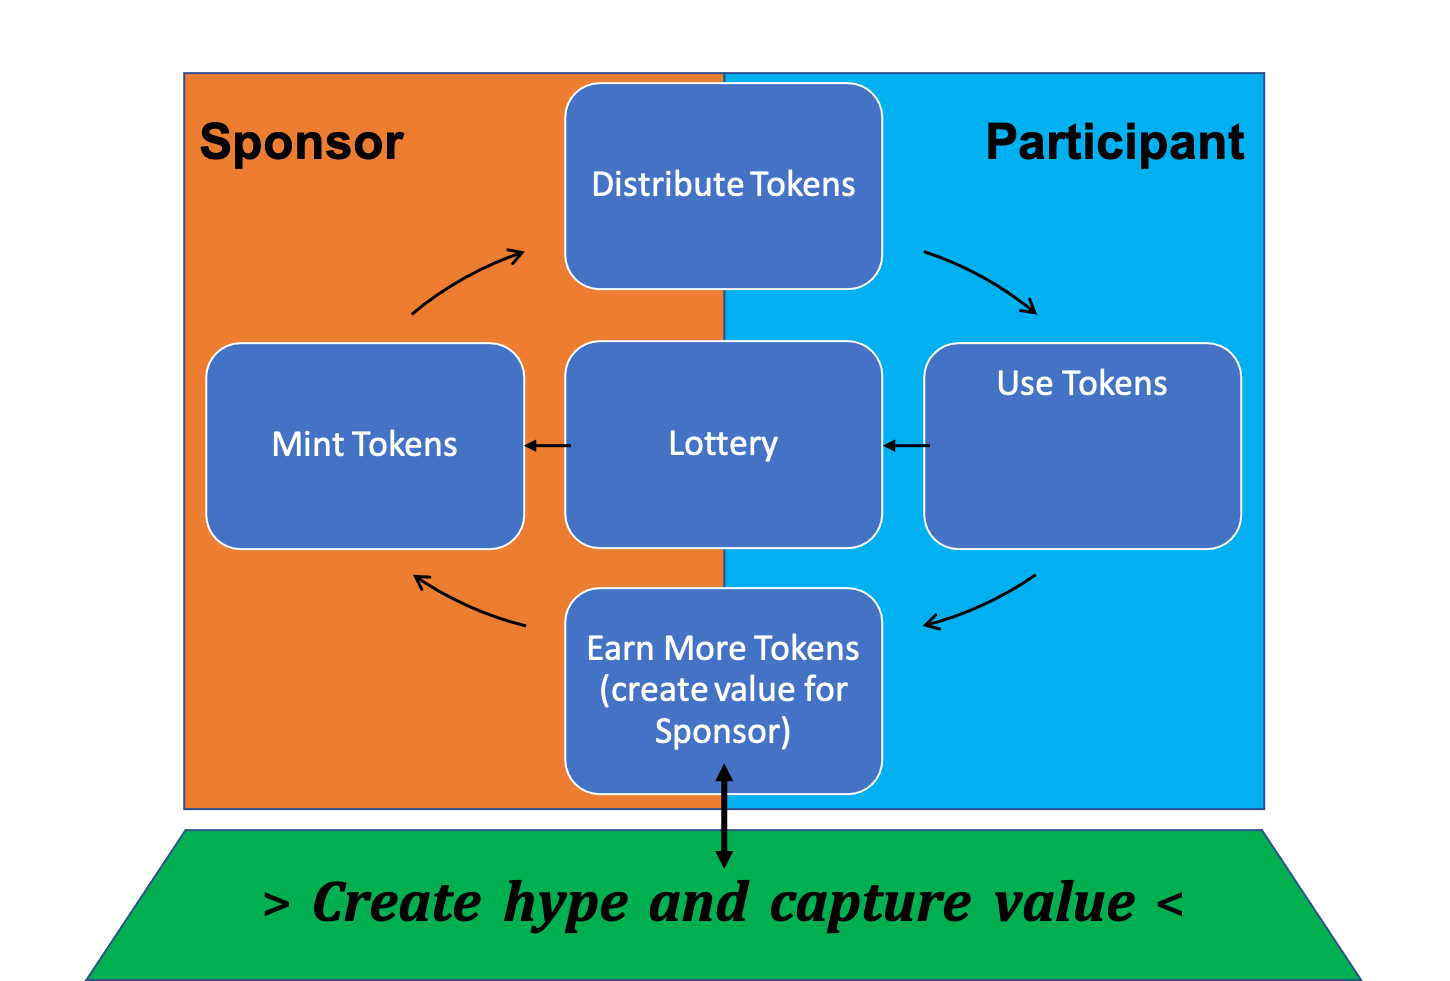
\includegraphics[scale=0.5]{Figures_and_Tables/Token_Value.png}
\caption{How Sponsor Tokens create Value.}
\end{figure}

\subsubsection{Sponsor Veracity and Reputation.}  As a decentralized platform, there is no centralized check on the authenticity of any information the Sponsor inputs to their profile.  Thus, the tradeoff to decentralization is that anyone can claim to be a brand.  A number of mechanisms are used to disincentivize and filter out bad actors from the platform.

First, we expect most Sponsors to use one wallet address for Lotteries and validate this address on verified social media accounts they control.\footnote{This can be simplified by Sponsor’s adopting ENS names.}   In addition, all users will have access to every Sponsor’s lottery history.  This history includes both rollups and details on individual lotteries, including number of entrants, total amount staked by Participants, and winning ticket details (the stakes and tokens). 

Sponsors are also encouraged to fully collateralize their lottery by locking value into the winning NFTs, discussed in subsection \ref{subsection-CreatingLottery}.

Additionally, there is a Reputational Scoring System which serves to verify the legitimacy of the Sponsor.\footnote{For a dApp platform without governance, the system needs to be secured purely through reputation.  As it evolves into a DAO, additional safeguards can be made through governance and other methods of verification.  For example, Sponsors can submit for Verification, or use a system such as the one used by Proof of Humanity, where other users stake value in support of a Sponsors claim at the risk of getting their stake slashed if it is determined they are working in collusion with a bad actor.}   It consists of two separate scores:

\begin{enumerate}
\item Distribution Score – This Score indicates the distribution of Sponsor Tokens (sum of all types) outside of the Sponsor’s Wallet.  This is important to show that the Sponsor is not concentrating Tokens in a few users, potentially indicating collusion between a Sponsor and certain Participants.  We use a modified GINI coefficient calculation to derive this score.  See Appendix \ref{APP-DistributionFunctions} for more information and a mathematical description of the Distribution Score.
\item Feedback Score – After participants win a lottery, they have the ability to give a simple positive signal back to the Sponsor.  Typically, this will occur after the winners redeem their item from the Sponsor.  Participants are incentivized to send the signal, however, as it helps the Sponsor whose assets they own and support.  The feedback score is a percentage of the number of positive signals divided by the total number of winners.  It omits any lotteries conducted within the previous three weeks to allow for fulfillment.    
\end{enumerate}

$$
\textrm{Feedback Score} = \frac{\sum \textrm{Positive Signals of the Winner}}{\textrm{Number of Total Winners} }
$$
% <<Feedback Score = ((Positive Signals from all Lottery Winners) / (Total Winners from all Lotteries)) * 100% | these do not include lotteries ending in the last 14 days>>

There is a third score that is less effective in determining Sponsor authenticity, but is an important characteristic of the Sponsor and helps them derive a metric-driven value from the platform.  It is called the Hype Score, and it is a measure of the difference between the sum of the Sponsors purses and the Total winning stakes the lotteries took in (called the lottery’s Residual, discussed in depth in \ref{subsection-ThePurseLotteryValuedStaked}).

$$
\textrm{Hype Score} = \frac{\sum \textrm{Total Winning Stakes for all Lotteries}}{\sum \textrm{Total Purses for all Lotteries}}
$$
%<<Hype Score = (Sum of total take from all Sponsor Lotteries) / Sum of Purses)

\subsection{Participants}\label{subsection-Participants}

Users access the Participant interface to enter a lotteries by staking value into a Sponsor’s lottery smart contract.\footnote{In the early days of the platform, a uniform cryptocurrency will be used for all transactions with the platform, both in and out.  It must be a stablecoin to ensure the values remain constant through the length of the lottery. However, at maturity, users will be able to swap any cryptocurrency for the Currency of Account set by the Sponsor, through an integrated swap mechanism directly on the platform.}

\subsubsection{Participant Interface and Dashboard.}  The Participant Interface and Dashboard includes:
User Settings
\begin{itemize}
\item Current Lotteries Participating in, to include time remaining and total amount staked
\item Lottery History 
\item Sponsor Tokens, and therefore Points, for Each Sponsor (with depreciation details)
\item Recommended Lotteries
\item Lottery Search/Browse
\end{itemize}
Unlike Sponsors, Participants have no external facing metrics on the platform.

\subsubsection{Sponsor Tokens}  The Sponsor and Participant must coordinate off-chain so the Sponsor has the Participant’s wallet address.  This shouldn’t be an issue as off-chain is where most of the discovery and value creation between Sponsors and Participants takes place.  Tokens increase the weight of a ticket, generally improving its odds of winning relative to a ticket with no/less tokens.  These tokens can be freely sold and traded.\footnote{From a brand’s perspective, issued Tokens have already created value for them, so they should not care who spends them.  While this may go against the notion of rewarding their biggest fans, most Participants will use their tokens themselves (or pool with friends to try and win an item) and also creates the potential to still capture value from the Drop by selling to others – which is aligned with the key aim of the platform.  Also, over time, it helps Sponsors determine their ticket weight factor parameters, as secondary token sales reveal their worth relative to money, and therefore price premium.}


\section{Lottery Process}\label{section-LotteryProcess}
Each Lottery is a smart contract – the Lottery Smart Contract (LSC).  It contains the Sponsor’s identity and the lottery parameters while holding the collateral, participants stakes, and the ticket pool.

In parallel to the LSC, a separate smart contract containing NFTs representing claims to the lottery items (be they physical or digital) is also created.  It is these NFTs that are transferred to the winners at the end of the lottery.

At the end date and time of the lottery (determined by the parameters), the smart contract acquires a random number from Chainlink’s VRF.  An off-chain deterministic function, living on multiple oracle nodes for decentralization, calls the random number and ticket data from the Lottery contract to determine the winners, and sends the list back on chain to both the LSC and the NFT contract.

\begin{figure}[H]
\centering
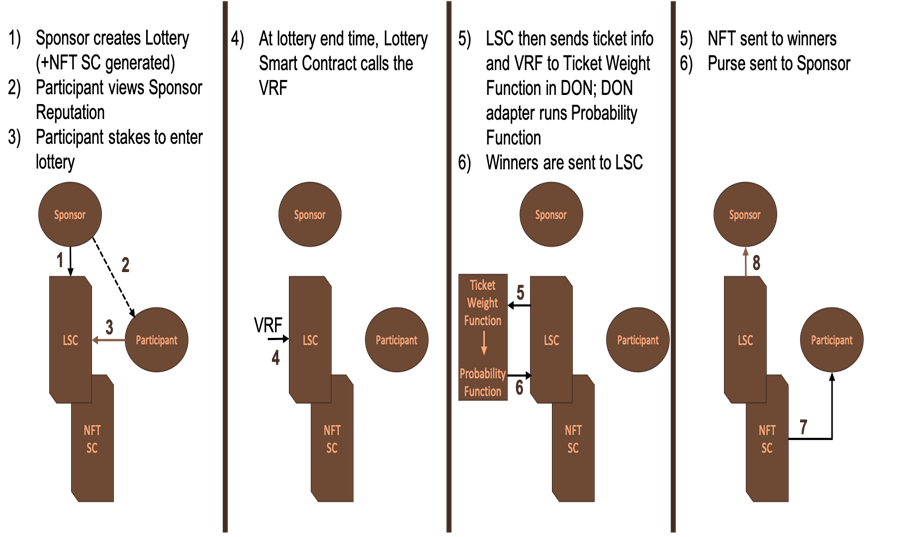
\includegraphics[scale=0.9]{Figures_and_Tables/LotteryProcessDiagram.png}
\caption{Lottery Process Diagram}
\end{figure}

\subsection{Creating a Lottery}\label{subsection-CreatingLottery}
A Sponsor determines the following lottery parameters which are encoded in the smart contract for that lottery:
\begin{center}
\begin{table} [h!]
\begin{tabular}{ |p{3cm}| p{8cm}| }
 \hline
 \textbf{PARAMETERS} & \textbf{DETAILS} \\ 
\hline
 Item Description & Includes Web2 links with images and more details  \\ 
\hline
 Lottery Duration & How long the lottery lasts, in time (lottery closes with closest block after this duration) \\ 
\hline
 Price of Item & Price Sponsor receives for each item, which is also the minimum stake price for the Participant. Includes the Currency of Account\tablefootnote{Currency of Account MUST be in a stablecoin or stable fiat currency.} \\
\hline
Quantity Available & Number offered, Q $\geq$ 1 \\
\hline
Sponsor Tokens Accepted & Which tokens the Sponsor will count towards ticket weight – can include other Sponsor-created tokens.\\
\hline
Collateral & How much money is locked into the winning NFT. \\
\hline
Fulfillment Details & A statement on how the Sponsor plans to trade the winning NFT for the good – be it physical or digital.  Will also include shipping restrictions – highly important! \\
\hline
Ticket Weight Function Parameters & Explained in detail in subsection \ref{subsection-Ticketing}\\
\hline
Redemption Period & How long after the lottery the winning NFT can be held or traded before it must be claimed.  After this time, a Sponsor could refuse to exchange for the good thereby forcing the holder to burn for any collateral locked into the NFT.  \\
\hline
(Optional) Start Date/Time & Lotteries can be triggered to start at a certain point in the future using Keepers.  Optional due to additional cost to implement. \\
\hline
\end{tabular}
\caption{Lottery Parameters}
\end{table}
\end{center}


\subsubsection{Collateral.}  Being an open platform, Sponsors are highly encouraged to collateralize their lotteries in order to give Participants some insurance for their stake.  This is achieved by locking value into each winning NFT at the creation of a lottery. A lottery is considered fully-collateralized if the value locked in each NFT is the same as the price of the good.\footnote{Note: This will not represent the total value staked for those winners who included a price premium.}   The collateral must be in the Currency of Account for the lottery.  

\subsection{Ticketing, the Pool and the Ticket Weight Factor}\label{subsection-Ticketing}
Once the lottery begins, be it manually triggered or at a set date and time through Keepers, Participants enter by staking a value equal to or greater than the item’s price into the lottery smart contract, thereby earning a chance to win an item.  This chance is represented by a ticket.  The ticket can include accepted Sponsor Tokens as well.  

\subsubsection{Stake Price Premium.}  The minimum stake required is the Price given by the Sponsor.  Additional value staked, called the Stake Price Premium, increases a ticket’s odds relative to a minimum stake.

\subsubsection{Determining Ticket Weights.} Ticket weight is a key aspect to the \textbf{DropShop} system.  Tickets are weighted, that is each ticket has a distinct probability of winning compared to other tickets staked for that lottery (other than those all weighted ‘1’ – which means no price premium or tokens include).  Collectively, these individual probabilities are collected into a pool.  Rather than one ticket, one chance, each ticket has a unique claim to a portion of the overall pool of entries. Ticket weight is determined by the Participants stake (in relation to the item price), the number of accepted Sponsor Tokens applied, and the Sponsor’s selection of how they want to weight the tickets themselves.

The last aspect – selection of how much price premium and tokens increase ticket weight - is determined by the Ticket Weight Factor (TWF), whose driving function’s parameters are selected by the Sponsor.  It is chosen by the Sponsor and drives an off-chain selection function run on oracles nodes.  As previously stated, the Participant has full visibility on the effects of the ticket weight function’s chosen parameters on a ticket’s weight.  An integrated tool can allow them to vary their intended stake and token amount to clearly see the effect on ticket weight before staking for a ticket.  The details and math behind the TWF can be found in Appendix \ref{APP-TWF}.

As most lotteries will have a quantity greater than one, when a ticket is selected as a winner, it is removed from the pool.

A Participant can stake for more than one ticket to win a lottery, with each ticket representing a separate chance to win a single item.  However, they will have to fully stake each, and tokens used for one ticket cannot be used in another.

One other important note: Sponsors can choose to accept \emph{any} other Sponsor’s tokens for the lottery, or choose not accept any Sponsor tokens at all (although this can also be achieved by eliminating their contribution to weight in the TWF).  This is especially useful in collaborations.  For example, a Yeezy X Supreme drop could choose to accept both Yeezy and Supreme tokens.

\subsection{The Purse, Take, and Residual}\label{subsection-ThePurseLotteryValuedStaked}
The sum of all winning stakes contained in a lottery’s smart contract is called the Lottery’s Purse.  The minimum Purse for a lottery’s must be its Quantity $\mathrm{Q}$ times the Price $\mathrm{P}$.  The product ($\mathrm{Q} \times \mathrm{P}$) is called the Take, and it is automatically transferred to the Sponsor at the lottery’s conclusion.

Most lotteries will have a Purse higher than the Take.  The difference is called the \emph{Residual} of the lottery.  The Residual is important because it can be distributed in a number of wars between the Sponsor, Participants and platform itself.  We discuss how the residual is used in greater detail in [\ref{section-PlatformEconomics}].

\subsection{Lottery Outcomes}\label{subsection-LotteryOutcomes}
At end time of the lottery\footnote{Technically the next block after the lottery duration ends.},  a 24-hour lockout period of the smart contract begins.  This is to ensure the platform can get some yield value while preventing the use of flash loans to spam a bunch of entries at the last minute. 

After the lockout period ends, Chainlink Keepers will check to ensure the minimum number of tickets have entered the lottery (simply the Quantity of the good offered) and if that passes calls the VRF, sends it and the ticket information to the probability function, and return the winners back.  If it fails for not meeting the minimum number of tickets, the lottery is invalidated and Participant stakes and any Sponsor collateral are returned.  

\subsubsection{Selection Function}.  The selection function is a probability function where the tickets are put into a pool and randomly selected, with their relative probabilities of selection determined by their TWF.  More details on the underlying math can be found with the TWF discussion in Appendix \ref{APP-TWF}

\begin{figure}[H]
\centering
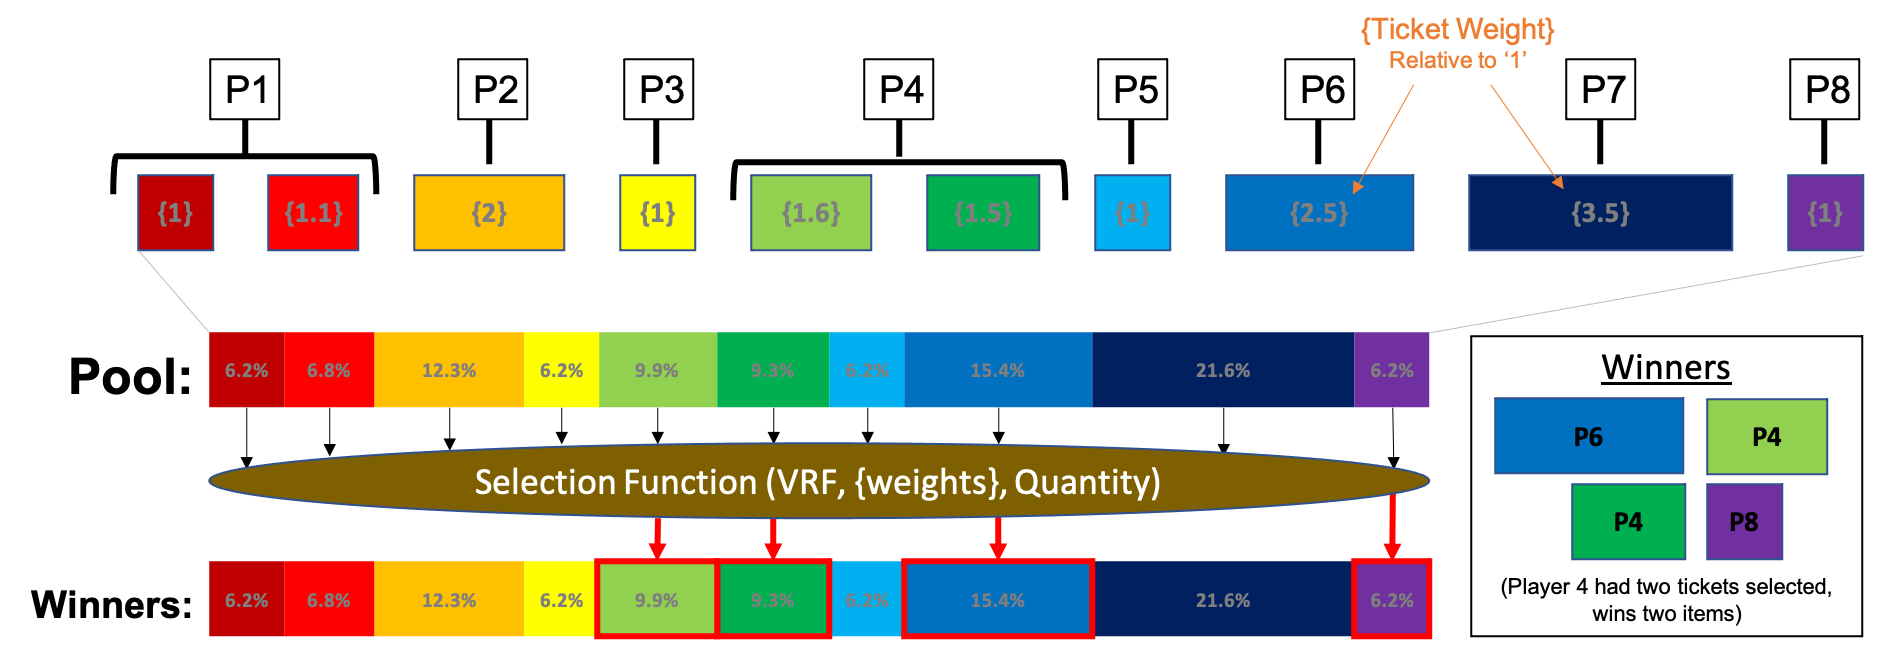
\includegraphics[scale=0.4]{Figures_and_Tables/Ticket_Pool.png}
\caption{Ticket Probability Pool and winner selection.}
\end{figure}

\noindent After winners are returned to the lottery smart contract the following occurs:
\begin{itemize}
\item Losing tickets will have their stake transferred back to the Participants wallets
\item Winners will receive an NFT representing an ownership claim to a lottery item from the Sponsor
\end{itemize}

\subsubsection{Return of Collateral, Sponsor Payment and Fulfillment.}  A critical challenge for this open, decentralized system is around Sponsor fulfillment and once the lottery ends, a particular challenge here since many of the lotteries will be for physical goods.\footnote{For digital goods, such as an NFT collection, this can be mitigated by creating a smart contract that holds and then releases both NFT once they are submitted.}   Since a winning Participant’s stake is already secured, fulfillment focuses on verifying the transmission of the good from the Sponsor to these winners.

For those Sponsors who collateralize the lottery, when the Participant trades the NFT for the item, the Sponsor can burn the NFT to recoup the value locked inside.  The participant can also burn it for the collateral if they feel the item will not be fulfilled.  It may be less than their stake as there is no protection for price premium, but it offers some insurance.  

There is still the risk that a Participant transfers their NFT to a Sponsor, who burns it to get their collateral back, but then does not fulfill the item.  Initially, users will have to rely on reputation and goodwill.  However, at maturity, we anticipate a robust ecosystem of automated supply chain tracking and management through blockchain and oracle systems.  The Sponsor and Participant will coordinate shipping of the good, either off-chain or through some sort of privacy maintaining on-chain method.  Chainlink Oracles or another service can then hold the Participant’s winning NFT in escrow until it verifies tracking information from the Sponsor (or runs the entire process itself), at which point the lottery smart contract releases the NFT to be burned to get collateral back.

There could also be physical vault services that can serve as custodial agents for lotteries, such as Mattereum.\footnote{See https://mattereum.com/}  They can take possession of the inventory from the Sponsor and then manage fulfillment.

Regardless of fulfillment method, once the Participant has received or sold their NFT, they are encouraged to give the Sponsor positive feedback (essentially a ‘thumbs up’) to improve the Sponsor’s reputation score.


\section{Platform Economics}\label{section-PlatformEconomics}

The platform derives value for itself primarily through staking assets held in lotteries and NFTs for yield.  This yield can then be funneled into a treasury smart contract within the platform.  In addition, a portion of the Residual can be captured by the platform as a fee for service.  

\subsubsection{Yield Farming.}  Stakes and collateral held within the platform can be used to generate yield (interest) through such platforms as 88mph and Aave, similar to a Lossless lottery such as PoolTogether.\cite{19}   An algorithm which takes into account inflows and outflows, along with the current level of the treasury, can maximize the amount used to generate yields and rebalance every 24 hours (lock out time post-lottery’s end).  

\subsubsection{Residual and the Treasury.}  Since all monies coming into the platform are in stablecoins, the treasury is in one or more stablecoins.  Here is the initial model we propose for distribution of the Residual:

\noindent Upon conclusion of the lottery, the Residual is distributed as follows:
\begin{itemize}
\item 25\% to the Platform treasury
\item 25\% to the Sponsor of the lottery
\item 25\% to the lottery winners, divided uniformly
\item 25\% lump sum to any participant (winner or loser), also determined by the VRF and unrelated to ticket weight
\end{itemize}

Alternatively, the Residual spend can be determined entirely by the Sponsor.  In this case, the platform should require a percentage of the Sponsor’s distribution go back to the platform and into its treasury. 


\section{Additional and Future Features}\label{section-FutureFeaturesGrowth}

\subsection{Secondary Marketplace}
A secondary market dominated by mass resellers using Bots is exactly what this platform seeks to mitigate.  However, a secondary market allowing primary consumers to resell goods should be supported.  It helps signal value and encourage hype for the Sponsor while the primary consumers of the good receive the most benefit from resale. 

\textbf{DropShop} will have an integrated Secondary market to allow for seamless resale of goods won for the duration allowed by the lottery parameters.\footnote{Non-redemption is a problem for Sponsors as they incur holding costs, hence the limits on secondary market duration in the parameters.}   Winning participants can port their winning NFT directly into the Secondary market.  These peer-to-peer marketplaces are well established in the NFT space already and would operate much like Opensea or Rarible.  It would allow for fixed price, timed auction or open bidding.

NFTs ported directly from the platform will have no service fees as both a reward and incentive for transacting on the platform.  The secondary market will be open to import and trade other NFTs, however they will be charged a service fee in the range of 1-5\%.

Non-redemption is a problem for Sponsors as they incur holding costs, hence the redemption period parameter which effectively limits secondary market duration.  Therefore, an NFT which passed it’s redemption period could be rejected by the Sponsor after this period, forcing the holder to burn and convert the NFT to its collateral – potentially lower than what was staked.

\subsection{Generalized User to User}
A generalized use-case of the platform’s mechanics include user-to-user, $\mathrm{Q} = 1$ transactions (in a primary market, not a secondary market as described above).    This feature would likely bifurcate from the drop lotteries, as they are a different class of value transaction.  

Sponsor metrics and Reputation scores would act as a rating system for the user as a whole.  

Auctions.  A natural extension for the platform would be to support auctions, be they created by a typical drop Sponsor, or a Participant user.  This functionality can be added through an auction smart contract suite.

\subsection{dApp to DAO}
Initially, the treasury will be a multisignature wallet managed by the creators.  However, the platform will likely move from a dApp to a DAO, and management will shift to holders of a Governance token.  This is the token that controls the protocol, including where to farm yield, and treasury distribution.  Any treasury distribution to holders would be released in proportion to one’s ownership of these tokens. 

Detailed mechanics are to be developed after initial dApp traction gained.


\section{Conclusion}
This paper presents \textbf{DropShop}, a blockchain-based lottery as a solution to the main complaint of limited release product drops – capture by resellers using Bots.

DropShop replaces these purely rent-seeking resellers with the end customer, who create hype value to compensate for the passive value creation by the inflated secondary market created by the Bots.

This hype is rewarded with Sponsor tokens, unique to the brand/company/service who create and distribute these tokens.  In turn, Sponsor tokens improve the probability of winning the lotteries in which they are accepted.  How they affect the probability, along with all of the other lottery parameters, are determined solely and transparently by the Sponsor.

DropShop uses Chainlink VRF for a verified random number to power its selection function which picks the winners.  This function is called through adapters to be executed on multiple oracles nodes, and returns a list of winners.  Winners receive an NFT claim to the asset and the Sponsor receives their Take for the lottery.  Any additional funds staked by the Participants is distributed according to current Residual distribution criteria.

Ultimately, DropShop can go beyond Drops to enable user to user asset transactions of any type – from secondary market transactions to primary market direct auctions and sales.


\section*{Appendix}
\appendix

\section{Distribution Functions}\label{APP-DistributionFunctions}


\section{TWF}\label{APP-TWF}


\section{Token Protocol}\label{APP-TokenProtocol}
This paper presents DropShop, a blockchain-based lottery as a solution to the main complaint of limited release product drops – capture by resellers using Bots.

DropShop replaces these purely rent-seeking resellers with the end customer, who create hype value to compensate for the passive value creation by the inflated secondary market created by the Bots.

This hype is rewarded with Sponsor tokens, unique to the brand/company/service who create and distribute these tokens.  In turn, Sponsor tokens improve the probability of winning the lotteries in which they are accepted.  How they affect the probability, along with all of the other lottery parameters, are determined solely and transparently by the Sponsor.

DropShop uses Chainlink VRF for a verified random number to power its selection function which picks the winners.  This function is called through adapters to be executed on multiple oracles nodes, and returns a list of winners.  Winners receive an NFT claim to the asset and the Sponsor receives their Take for the lottery.  Any additional funds staked by the Participants is distributed according to current Residual distribution criteria.

Ultimately, DropShop can go beyond Drops to enable user to user asset transactions of any type – from secondary market transactions to primary market direct auctions and sales.

\
\paragraph*{Acknowledgements} 
The authors warmly thank the ChainLink team for sharing historical price feed addresses with us for cross-verification. \textbf{to be edited}

% ---- Bibliography ----
%
% BibTeX users should specify bibliography style 'splncs04'.
% References will then be sorted and formatted in the correct style.
%
% \bibliographystyle{splncs04}
% \bibliography{mybibliography}
%

% \bibliographystyle{splncs04}
% \bibliography{references}



\end{document}
